\documentclass{sig-alternate}

\begin{document}

 \conferenceinfo{GECCO'15,} {July 11-15, 2015, Madrid, Spain.}
    \CopyrightYear{2015}
    \crdata{TBA}
    \clubpenalty=10000
    \widowpenalty = 10000

\title{Novelty Search of Soft Robot Morphologies for Space Exploration}
%\subtitle{[Extended Abstract]
%\titlenote{A full version of this paper is available as
%\textit{Author's Guide to Preparing ACM SIG Proceedings Using
%\LaTeX$2_\epsilon$\ and BibTeX} at
%\texttt{www.acm.org/eaddress.htm}}}

\numberofauthors{1}
\author{
\alignauthor
???
% \alignauthor
% Ben Trovato\titlenote{Dr.~Trovato insisted his name be first.}\\
%       \affaddr{Institute for Clarity in Documentation}\\
%       \affaddr{1932 Wallamaloo Lane}\\
%       \affaddr{Wallamaloo, New Zealand}\\
%       \email{trovato@corporation.com}
% % 2nd. author
% \alignauthor
% G.K.M. Tobin\titlenote{The secretary disavows
% any knowledge of this author's actions.}\\
%       \affaddr{Institute for Clarity in Documentation}\\
%       \affaddr{P.O. Box 1212}\\
%       \affaddr{Dublin, Ohio 43017-6221}\\
%       \email{webmaster@marysville-ohio.com}
% % 3rd. author
% \alignauthor Lars Th{\o}rv{\"a}ld\titlenote{This author is the
% one who did all the really hard work.}\\
%       \affaddr{The Th{\o}rv{\"a}ld Group}\\
%       \affaddr{1 Th{\o}rv{\"a}ld Circle}\\
%       \affaddr{Hekla, Iceland}\\
%       \email{larst@affiliation.org}
% \and  % use '\and' if you need 'another row' of author names
% % 4th. author
% \alignauthor Lawrence P. Leipuner\\
%       \affaddr{Brookhaven Laboratories}\\
%       \affaddr{Brookhaven National Lab}\\
%       \affaddr{P.O. Box 5000}\\
%       \email{lleipuner@researchlabs.org}
}

\maketitle
\begin{abstract}
don't worry about this, we gonna write it at the end
\end{abstract}

% A category with the (minimum) three required fields
\category{H.4}{Information Systems Applications}{Miscellaneous}
%A category including the fourth, optional field follows...
%\category{D.2.8}{Software Engineering}{Metrics}[complexity measures, performance measures]

\terms{Theory}

\keywords{soft robotics, novilty search, CPPN, HyperNEAT, VoxCAD}

\section{Introduction}
Motivation, space, small bodies, passive actuation, story of Rosetta/Philae - stupid rigid probe without locomotion, we can do better!

\section{Background}
\begin{itemize}
\item gaits at different gravity levels (Ariadna Space Gaits); fixed morphology, rigid body dynamics
\end{itemize}
\subsection{Soft Robots}

Soft robotics is a highly promising field of research dedicated to the science and engineering of soft materials in mobile machines. As the name suggests soft robots~\cite{trivedi2008soft, pfeifer2012challenges} are made entirely of soft materials mimicking animals or animal-parts that consist only of soft tissue (elephant trunk, tongue, worm, octopus, etc.). Having no rigid parts in their design the degrees of freedom are infinite and the possible ways of motion can become extremely complex. In traditional robotics, joints and rigid parts predefine the space of possible movement and sometimes restrict the robot's locomotion strategy or \emph{gait} to a specific set. In soft robotics, the absence of rigid parts can on the one hand make the design of the locomotion strategy exceptionally tortuous, on the other hand the gait alternatives are limitless.

\begin{figure}[h!]
\centering
\includegraphics[width=0.15\textwidth,height=0.09\textheight]{../Figures/Misc/soft_robotics_figure.png}\		
\includegraphics[width=0.15\textwidth,height=0.09\textheight]{../Figures/Misc/hillerPressureChamber.png}\	
\includegraphics[width=0.15\textwidth,height=0.09\textheight]{../Figures/Misc/ExplodingRobot.jpg}\\
\caption{Soft robots can be actuated through air pressure tubes (left), pressure variations (middle), or internal explosions (right).}
\label{fig:softRobotsActuation}
\end{figure}

The design and development of soft robotics is not an easy task, while the actuation of such soft structures is the most challenging task. Actuating soft materials can be done in many ways including pneumatic systems~\cite{ilievski2011soft, shepherd2011multigait}, hydraulic, internal body explosions, passive actuation triggered by pressure or temperature variations and others~\cite{laschi2012soft, seok2010peristaltic}. Figure~\ref{fig:softRobotsActuation} illustrates four different ways that soft robot bodies can be actuated. Regardless traditional ways of actuating soft material robots, three dimensional printing is now giving the freedom for multi-material structures to be created, which also explodes the number of possibilities for the design of a soft structure robot. Autonomously actuated soft robots~\cite{tolleyresilient} (see Fig.~\ref{fig:softbot}) can also be designed having multiple advantages over rigid body robots such as resistance under extreme temperatures and the capability of locomotion on terrains of variant types.

\begin{figure}[b!]
\centering
\includegraphics[width=0.3\textwidth]{../Figures/Misc/softbot.jpg}
\caption{Autonomously actuated soft robot~\cite{tolleyresilient}, it is able to withstand extreme temperatures and variant terrain types.}
\label{fig:softbot}
\end{figure}

Although soft robotics research field is in an early stage, it is growing fast. Some of the characteristics that make soft robots interesting to explore are the infinite number of degrees of freedom and the variety of materials (mostly elastic) that can be used, in the contrary to rigid robotics that are mostly made out of metals and plastic. Nevertheless, structure design and control of soft robotics remain challenging mostly because of their soft bodies can only be represented in continuous state spaces, where only analytic methods can be proven successful.


\subsection{Evolution of Soft Robots}

Topological optimization techniques can be applied to soft robots~\cite{hiller2009multi} for producing functionality in the design. Evolution of soft material robots as it was shown in~\cite{hiller2012automatic}, can result in soft robots able to produce locomotion. The possibility of evolving these soft structures using an indirect encoding was of interest to be exploited by~\cite{cheney2013unshackling}. A powerful generative encoding, CPPNs~\cite{stanley2007compositional}, was used to generate soft voxel-formed three-dimensional structures, coupled with the use of NEAT algorithm which ensures the increasing complexity of the networks produced. The superiority of this kind of generative encoding was verified against direct encoding, showing how CPPNs can take advantage of their geometrical properties. Evaluation was done by a simple displacement measure while evolution tended to evolve different kinds of locomotion strategies and morphologies as the fitness function was penalized for different parameters. Furthermore, it has been shown that evolving morphologies (CPPNs) in lower resolutions and then applying the same networks for higher resolution structures can be beneficial, since the locomotion behaviors in lowers structures also apply in higher saving computational time. An earlier work~\cite{hiller2010evolving}, apart from the generative encoding of CPPNs, made use of \textit{Gaussian Mixture} and \textit{Discrete Cosine Transform} to produce amorphous soft body structures. The simultaneous evolution of soft robot morphology and control was also investigated by recent work~\cite{rieffel2014growing}. Some aspects of soft robot evolution were verified in this work, namely muscle placement and muscle-firing patterns can be evolved given a fixed body shape and fixed material properties. Furthermore, material properties can be co-evolved alongside locomotion strategies. Finally, a developmental encoding was introduced, allowing more complex parts to be added to soft robotic structures during the evolution.

\section{Methodology}
\subsection{VoxCAD simulator}

\begin{figure}[t!]
\centering
\includegraphics[width=0.4\textwidth]{../Figures/Misc/voxcad.png}
\caption{VoxCAD (Voxel CAD), a cross-platform open source voxel modeling and analyzing software.}
\label{fig:VoxCAD}
\end{figure}


Most work to simulate interactions and deformations within and between soft material bodies are mostly focused on the graphical part of the problem~\cite{faloutsos1997dynamic} sacrificing the accuracy of the simulation~\cite{teschner2004versatile}. Three dimensional meshes~\cite{muller2002stable} can represent these bodies including the dynamics of their materials. 

A recent work, \emph{VoxCad} simulator~\cite{hiller2012dynamic}, is focusing mostly on the physics side of the soft material interactions not at the expense of a low frame rate. VoxCad is a modeling and analyzing open-source software that can simulate soft material deformations and interactions. In Figure~\ref{fig:VoxCAD} the graphical user interphase of VoxCad software is presented during the simulation of the soft body robot in the simulator.

VoxCad cannot model and simulate three dimensional meshes, yet a lattice is used to represent the 3D workspace where voxels (three dimensional pixels) can be assigned different materials. Materials themselves are passive and cannot actuate without external trigger. In this simulator this external force that can actuate the materials is the temperature of the environment. The main variables of the environment is the base, the amplitude and the period of the temperature. Materials have properties such as the elasticity of the material, density, Poisson's ratio, coefficient of thermal expansion (which determines how materials will be expanded in respect to the environment's temperature), temporal phase in respect to the temperature period, and the ground friction coefficients. Materials can also be mixed together to create a new type of material. Furthermore, gravity acceleration of the environment can vary.

\subsection{Compositional Pattern-Producing Networks}

\begin{figure}[b!]
\centering
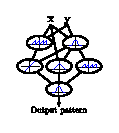
\includegraphics[width=0.15\textwidth]{../Figures/Misc/cppnNetwork.eps}
\caption{Compositional pattern-producing networks have identical network structure with artificial neural networks while they make use of a canonical set of activation functions.}
\label{fig:cppnNetwork}
\end{figure}

\emph{Compositional pattern-producing networks}~\cite{stanley2007compositional} or CPPNs are artificial neural networks with an extended set of activation functions (see Fig.~\ref{fig:cppnNetwork}). This set of activation functions include repetitive, symmetrical, and linear functions as it is shown in the previous figure. Results by this encoding show that regular patterns can be produced in this generative mapping from the genotype to the phenotype space. CPPNs can generate phenotypes that can be interpreted as distributions of points in a multidimensional Cartesian space. The genotype (CPPN) can then be queried for each coordinate of the space and gives the phenotype representation of the genotype in multiple resolutions. In the same fashion, images can be constructed using CPPNs, where pixel coordinates are queried to the network and the grayscale or RGB values can be taken by the outputs of these networks. 

Figure~\ref{fig:cppnResolution} illustrates how the mapping between the genotype and phenotype is done using this type of generative encoding (CPPNs). A major asset of CPPNs is that they can generalize in all resolutions. Considering the previous figure (see Fig.~\ref{fig:cppnResolution}), the CPPN is queried for all $x,y$ coordinates of the phenotype two dimensional Cartesian space. The step of $x,y$ sampling can be determined by the problem, since the inputs of the CPPN are the normalized coordinates $x,y \in [-1,1]$. Hence, genotypes using this kind of generative encoding can be mapped in every resolution, making this process straighforward to generalize. As the space of the phenotype becomes larger, a generative encoded solution (CPPN) is not affected by the increasing dimensions of the problem, a constraint that heavily affects direct encoding.

\begin{figure}[t!]
\centering
\includegraphics[width=0.3\textwidth]{../Figures/Misc/cppnResolution.eps}
\caption{CPPNs work as a function $f$ that is being queried for the whole n-dimensional Cartesian space in which space the phenotype is mapped, in this case the phenotype is the triangle in a two-dimensional space, figure taken by~\cite{stanley2007compositional}.}
\label{fig:cppnResolution}
\end{figure}

\subsection{Neuroevolution of Augmented Topologies}

Neuroevolution of augmented topologies (NEAT) as it was first introduced by~\cite{stanley2002evolving} is a neuroevolution method to evolve artificial neural networks. A major advantage of this method is that alongside the weights it also evolves the topologies of the networks within the population.

Originally, neuroevolution methods were developed to capture difficult sequential decision making, as well as to control problems. The sensory information is the input of these neural networks and decisions are the outputs. NEAT is yet another method for evolving ANNs where a few extra features are added, enables finding solutions in more demanding problems. NEAT starts the evolution process with a population of networks with simple topologies. Through the generations instead of just fixing the weights of the networks' connections, topologies are becoming more complex allowing nodes and links to be added. Meaning that during the evolution, more complicated networks will be produced, this \emph{complexifying} technique leads to capturing more demanding solutions as it offers enough freedom to the evolution.

Several aspects of this method worth mentioning where \emph{speciation} is one of the most important. Speciation is the procedure that protects new \emph{species} until they have enough time to evolve before comparing them with the rest of the population. For two individual genotypes (ANNs) to belong to the same species their network topology must be similar, meaning that a threshold is set and a function determines the numeric value of two network topologies' similarity. Two different genotypes (ANNs) can share shame genes (topologies within the network) and their compatibility (genotype similarity) is given by:
\begin{equation}
\label{CompatibilityEquation}
\delta = c_1 \cfrac{E}{N} + c_2 \cfrac{D}{N} + c_3 \bar{W}
\end{equation}
where $E$ is the number of \emph{Excess} genes (genes that do not match and they do not occur in parents' genotype), $D$ is the number of \emph{Disjoint} genes (genes that do not match but they occur in parents' genotype), $\bar{W}$ is the average weight difference between \emph{Matching} genes (Identical) and $N$ is the number of genes in the larger genotype used for normalization.

The age of each species protects them for competing in equal terms with more optimized species, giving them in this way time to evolve further towards the objective function.


\subsection{CPPN-NEAT}

Compositional pattern-producing networks as described earlier are similar computational methods to ANNs in regards to their structure, so one can make use of the \emph{complexifying} property to capture in this way more complex solutions. NEAT method can evolve CPPNs in the place of ANNs, since it only needs few modifications. 

The resulted method that evolves this generative type of genomes (CPPNs) is called CPPN-NEAT~\cite{stanley2007compositional} and its only difference in respect to the original NEAT algorithm is the way new nodes are added to the network. The original NEAT algorithm evolves ANNs which are using sigmoid functions at every node, so every new node will carry this function.
In the contrary, CPPNs use a variety of functions from a canonical set. CPPN-NEAT assigns a random function from this set to every newly added node. 

Experiments~\cite{stanley2007compositional} have shown that this method can indeed evolve CPPNs capturing in this way solutions in problems with geometrical properties (i.e board games, biped walking, etc.). NEAT is holding the properties of natural evolution as every neuroevolution method. Furthermore, NEAT coupled CPPN encoding can be used to determine the connectivity (topology) of artificial neural networks in  a method called HyperNEAT~\cite{stanley2009hypercube}.


\subsection{Novelty search}

Novelty search~\cite{lehman2008exploiting,lehman2011abandoning,lehman2010revising, risi2009novelty} unlike traditional fitness based search is an alternative way of optimization towards an objective function without having knowledge of this objective. In simple words it is looking for a solution to a problem without knowing how close it is to solve it; fact that turns out to have a major impact to the increased performance of this method in several problem domains. 

What novelty search seeks for is how interesting a new solution is in respect to all previously found ones. To define ``interesting'' we need to move our point of interest into behavior space which is a function of each phenotype, similar to the fitness function. Nevertheless, it fully or partially describes the behavior without directly implying the fitness function. As an example someone can think of a behavior could be defined as the recorded trajectory of a robot which tries to maximize its velocity. Rewarding behaviors of the phenotype that are different from the previously found ones drives the evolution to visit new points in the behavior search space.

One significant point here is that the behavior space in some domains can be limitless. However, a valid behavioral metric can be found excluding behaviors that are meaningless or do not comply with the natural limits of the problem. On the other hand, the search space in the genotype level can also be infinite especially in neuroevolution methods like NEAT where ANNs can grow during the evolution. A bounded space of understandable-valid behaviors is then the key idea of novelty search where increasingly complex behaviors present to the evolution as the complexity of the genotype grows along.

Multi-objective optimization can also make use of a novelty metric alongside fitness, trying to optimize both at the same time~\cite{mouret2011novelty}. Another method that exploits the diversity of the produced genomes in order to map the phenotype to the fitness has also been proposed~\cite{mouret2012algorithm}.

\subsubsection{Behaviours}

\begin{figure}[h]
\centering
\includegraphics[scale=0.19]{../Figures/Behaviors/3d.pdf}\includegraphics[scale=0.18]{../Figures/Behaviors/2d.pdf}
\caption{Observed behaviors of the soft robots used for the sparsity computation in novelty search.}
\label{fig:Behaviors}
\end{figure}

\emph{Behavior} can be defined as the way that a human/machine behaves towards or within an environment. Regarding the evolution of soft robots in the specific simulated environment, a behavior can be defined as the way soft robots behave in respect to their locomotion strategy. Every aspect of the soft robots movement that can be observed can be used to describe their behavior. Previous work~\cite{lehman2011evolving} in a try to evolve walking three-dimensional virtual creatures used the evolved morphology of the creatures to describe their behavior. Although, in this work comparing the morphology of the evolved soft robots is similar to comparing the chromosome (CPPN) of each individual. Therefore, only the comparison of the observed behavior in phenotype level can lead the evolution towards more complex behaviors.

A straightforward function that determines the goodness of an individual is used in fitness based methods. This measure drives the search in ``good'' areas of the search space. However, the same measure cannot be used for novelty search. What novelty search looks for is novelty in behavior space. It is expected that behaviors that contain information about the goodness (displacement) of individuals will be more successful than behaviors that include other aspects of the soft robots' behavior. In cases that behavior does not contain information about the objective, the search for novelty will become random in regards to this objective function.

Behaviors that describe the morphology of the evolved robots have failed~\cite{lehman2011evolving}, since search is then forcing new types of morphologies without caring about the actual target of the evolution, which was the efficient locomotion. To present a similar idea consider a behavior metric that enumerates the number of voxels a soft robot consists of. This is not a well-founded behavior metric, since the search will reward new structures with different number of voxels from previous evolved structures. Therefore, there will not be exploration in the behavior aspect that affects the actual target of the evolution, which is to produce and evolve efficient locomotion strategies.

Figure~\ref{fig:Behaviors} presents all behaviors used for the novelty metric computation together with the sampling rate of the recorded values during the simulation and their description. For all recorder behavior metrics a constant sampling rate ensures that all signals have the same length. The behaviors designed to describe the strategy and the efficiency of the evolved  locomotion. They contain information that indirectly implies both the objectives of the evolution. \emph{Trajectories} (2D and 3D), incorporate all the needed information such as speed, displacement, and locomotion strategy. To avert from same trajectories in all possible directions trajectories are normalized, meaning that their starting coordinates are always the start of the axes ($<0,0,0>$) and the point coordinates of the trajectory are rotated so their center of mass is normalized to a specific angle ($\theta = 90^{o}$). To measure the difference of two trajectories the Euclidean distances between coordinates at the same sampling time are measured, so that:
\begin{align}
\text{First trajectory: } &t_i = t_i^1, t_i^2, \ldots, t_i^N\\
\text{Second trajectory: } &t_j = t_j^1, t_j^2, \ldots, t_j^N\\
\text{Difference: } &t_i - t_j = \sum_{n=1}^{N} dist( t_i^n, t_j^n )
\end{align}
where $n$ is the number of sampled coordinate points and $dist$ is the Euclidean distance. \emph{Pace} is also a very informative behavior metric as it directly measures the speed of the robot. \emph{Voxels touching the ground} can also imply information about the locomotion strategy but not enough about the actual performance regarding the displacement. Hopping robots that move fast can have same behaviors with regards to this metric with hopping robots with zero speed. \emph{Maximum pressure} among the voxels' connection is yet another behavior metric, pressure is expected to become higher as structures move faster and interactions with the ground eventually getting harder. Finally, \emph{maximum kinetic energy} is a behavior metric that straightly determines the displacement of the voxels in the structure. To compute the difference between two signals, a straightforward method is used. Subtracting the one signal from the other, taking the absolute differences, and summing them up to compute one single value that describes how variant the two signals are. More specifically:
\begin{align}
\text{First 1-d signal: } &s_i = s_i^1, s_i^2, \ldots, s_i^N\\
\text{Second 1-d signal: } &s_j = s_j^1, s_j^2, \ldots, s_j^N\\
\text{Difference: } &s_i - s_j = \sum_{n=1}^{N} | s_i^n - s_j^n |
\end{align}
For all behaviors but trajectories, the Fourier profile of their signals can also be used as an observed behavior. This process of transformation of the one-dimensional signals into frequency space eliminates shifts of signals in time-axis. The discrete Fourier transformation:
\begin{equation}
C_i^k = \sum_{n=1}^{N} s_i^n e^{-i 2 \pi k n/N,},~\forall k \in \mathbb{Z}
\end{equation}
For the Fourier transformations of these signals the first twenty coefficients are compared, and the summation of their absolute differences determines the difference of the two behaviors.
\begin{equation}
\text{Difference in frequency: } s_i - s_j = \sum_{k=0}^{R-1} | C_i^k - C_j^k |, R=20
\end{equation}

In this section, different observed behavior metrics have been defined. The similarity or difference of two same type behaviors can be determined by the equations provided while these measures of difference are used by the sparsity equation (see Eq.~\ref{sparsenessEquation}) to compute the sparseness of a given behavior in the behavior space. Individuals with novel observed behaviors (high sparseness value) are then stored in a list helping the evolution to avoid generating similar behaviors (see Alg.~\ref{noveltyPseudocode}).

\subsection{Novelty + Fitness-based}

\subsection{Experimental setup}
parameters, gravity

\section{Results}
novelty (+ fitness) better than fitness
examples of cool creatures
taxonomy of the evolved creatures at different gravity levels (hoppers, 2-3-4 legs, crawler, tumbleweed) 

\section{Discussion}
what's the use of this?
getting inspiration for soft robotic probe / landers (tumbleweed)
come back to asteroid scenario (passime motion), would it have saved Philae?

\section{Conclusions}
our setup better than results from "unshackling evoltion"
methodology is suitable to design diverse gaits of soft robots at various gravity levels
future work: ensamble of behaviors, very low gravity environments and rotational parameters of small body linked to actuation frequency

\bibliographystyle{abbrv}
\bibliography{bibliography}

\end{document}
